%!tex engine=xelatex
\documentclass[a4paper]{article}

\usepackage[margin=1.5in]{geometry}
\usepackage{amsmath,amssymb}
\usepackage{aastexmacros}
\usepackage{graphicx}
\usepackage{hyperref}

\usepackage{natbib}
\bibliographystyle{unsrtnat}

\usepackage{fontspec}
\setmainfont{EB Garamond}

\newcommand{\defn}[1]{\emph{#1}}

\title{Measuring Faraday Complexity}
\author{Matthew J. Alger\\{\small Research School of Astronomy and Astrophysics, ANU}\\{\small Data61, CSIRO}}

\begin{document}
    \maketitle

    \section{The Faraday Effect}

    The \defn{Faraday effect} is the rotation of light as it passes through a magnetic field. The amount of rotation is wavelength-dependent. This rotation and its variation over wavelengths can be measured with radio telescopes, giving us insight into physical processes between the source and the observer.

    Linear polarisation $P$ can be decomposed as the Stokes $I$, $Q$ and $U$ parameters following \citet{burn66depolarization} and \citet{bell12faraday}:
    \[
        P(\lambda) = Q(\lambda) + iU(\lambda) = \int_{-\infty}^{\infty} e^{2i\phi\lambda^2} F(\phi)\ d\phi.
    \]
    $\phi$ is the \defn{Faraday depth}, measured in $\mathrm{rad}\ \mathrm{m}^{-2}$. This is interpretable as a measure of how much rotation an intervening medium gives to an intrinsic polarisation angle as a linear function of $\lambda^2$. Note that this looks a lot like a Fourier transform of $F(\phi)$, which we call the \defn{Faraday spectrum}. For a simple source with rotation at just one Faraday depth $\phi_0$, $F(\phi) = \delta(\phi - \phi_0)$ and
    \begin{align*}
        P(\lambda) &= \int_{-\infty}^{\infty} e^{2i\phi\lambda^2} \delta(\phi - \phi_0)\ d\phi\\
            &= e^{2i\phi_0\lambda^2}\\
            &= \cos (2\phi_0\lambda^2) + i \sin (2\phi_0\lambda^2).
    \end{align*}
    We can then identify $Q = \cos(2 \phi_0 \lambda^2), U = \sin(2 \phi_0 \lambda^2)$ and hence the polarisation angle $\chi$ can be written
    \[
        \frac{1}{2} \mathrm{arctan}\ \frac{U}{Q} = \phi_0 \lambda^2,
    \]
    i.e. $\phi_0$ is the gradient of the polarisation angle as a function of $\lambda^2$. This relationship holds more generally for a quantity called the \defn{rotation measure} $RM$ which is equal to $\phi_0$ only for this simple case:
    \[
        RM = \frac{\partial \chi}{\partial \lambda^2}.
    \]

    We can write the Faraday depth of the point $r$ (with respect to an observer at $r = 0$) in physical terms $\phi(r)$ is the \defn{Faraday depth} of the point $r$ (with respect to an observer at $r = 0$). The Faraday depth carries physical meaning, with
    \[
        \phi(r) = \frac{e^3}{2\pi m_e^2 c^4} \int_0^r n_e(l) B_{||}(l)\ dl.
    \]
    $n_e$ is the electron density and $B_{||}$ is the line-of-sight magnetic field strength. $\phi$ is measured in $\mathrm{rad}\ \mathrm{m}^{-2}$.

    \begin{figure}
        \centering
        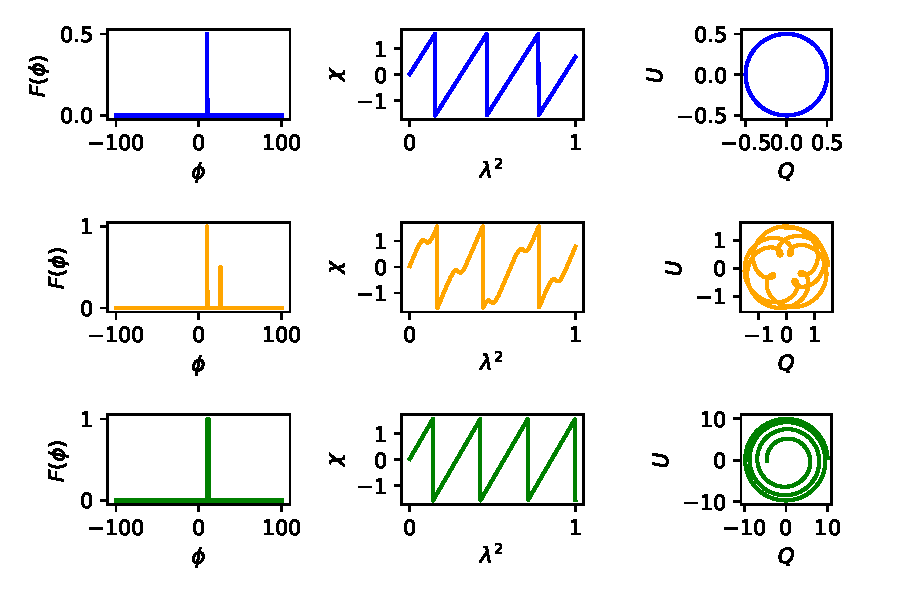
\includegraphics[width=0.8\textwidth]{faraday-depth.pdf}
        \caption{Different Faraday depth distributions (left) lead to different polarisation spectra (centre) and different-shaped $Q$/$U$ plots (right). Here we show a Faraday screen (top), two Faraday screens (centre), and a Faraday slab (bottom). \label{fig:faraday-depth-models}}
    \end{figure}

    More complex models are commonly applied. These are usually combinations of tophat and delta functions. Some of these models are shown in \autoref{fig:faraday-depth-models}.

    \section{Faraday Complexity}

    \defn{Faraday complexity} is a measure of how complex a polarised Faraday spectrum is. It's unclear exactly what a good Faraday complexity metric would look like, but at minimum a spectrum can be \defn{Faraday simple} if it is well-fit by a single Faraday screen. A spectrum that is not Faraday simple is then \defn{Faraday complex}. Perhaps we could even have some kind of `score', where higher numbers indicate `more' Faraday complexity.

    \bibliography{faraday-complexity}


\end{document}